\documentclass[11pt]{article}
\usepackage{float}
\usepackage{amssymb}
\usepackage[english]{babel}
\usepackage{fullpage}
\usepackage{graphicx}
\usepackage{hyperref}
\usepackage{pythonhighlight}
\usepackage{listings}
\usepackage{ragged2e}
\usepackage{listings}

\def\titre{}
\def\auteur{}
\def\courriel{}
\makeatletter

\title{Polytechnique Montreal\\LOG8415 : Advanced Concepts of Cloud Computing\\Laboratory 2\\MapReduce with Hadoop on AWS}


\author{
    Christian Njon\\
    Dimitry Kamga\\
    Michelle Sepkap Sime\\
    Rui Jie Li
}

\date{4th November 2022}


\begin{document}
\maketitle

\maketitle

\section{Introduction}
MapReduce on Hadoop and Spark using AWS is the subject of the second assignment for the LOG8415E course. The objectives of this assignment are to acquire some skills with large data technologies and learn to integrate issues and methods into the MapReduce paradigm. Four primary sections make up this report. First, we will discuss our Word Count application in Hadoop trials. Second, we compare Hadoop's performance to that of Linux. Third, we compare the performance of Spark and Hadoop on AWS. We wrap up by outlining our algorithm and the MapReduce tasks we used to tackle the social network problem. We present our recommendations for connections based on the algorithm.

\section{Hadoop and Spark}

\subsection{Experiments with Word count Program}
Here, we first prepare the lab setting by setting up Hadoop on our computer. We adhered to the assignment's guidelines. Our major goal was to use Hadoop to process a pg4300.txt file. So that the Hadoop Name Node and Data Nodes could share the file, we downloaded it to a local directory and then moved it to the Hadoop Distributed File System (HDFS).
The data file pg4300.txt was then moved to the "input" directory we had just created in the Hadoop Distributed File System (HDFS).
The wordcount.java program from the Hadoop example directory was then executed. The screen capture of the Hadoop settings on localhost is shown in Figure~\ref{fig:hadoopgui1} and Figure~\ref{fig:hadoopgui2}. The input directory containing the pg4300.txt file is shown in Figure~\ref{fig:hadoopgui3}.

\begin{figure}
    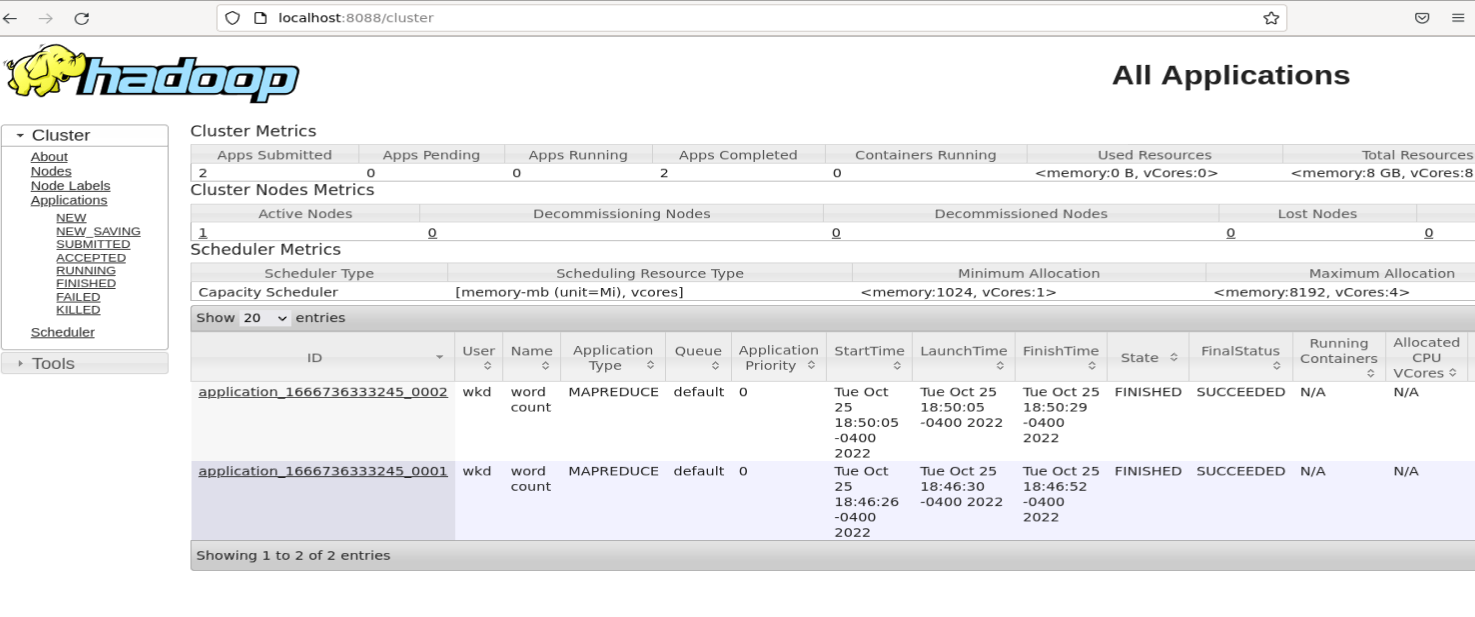
\includegraphics[width=\linewidth]{hadoop_gui1.png}
    \caption{Hadoop Overview GUI - part1}
    \label{fig:hadoopgui1}
\end{figure}

\begin{figure}
    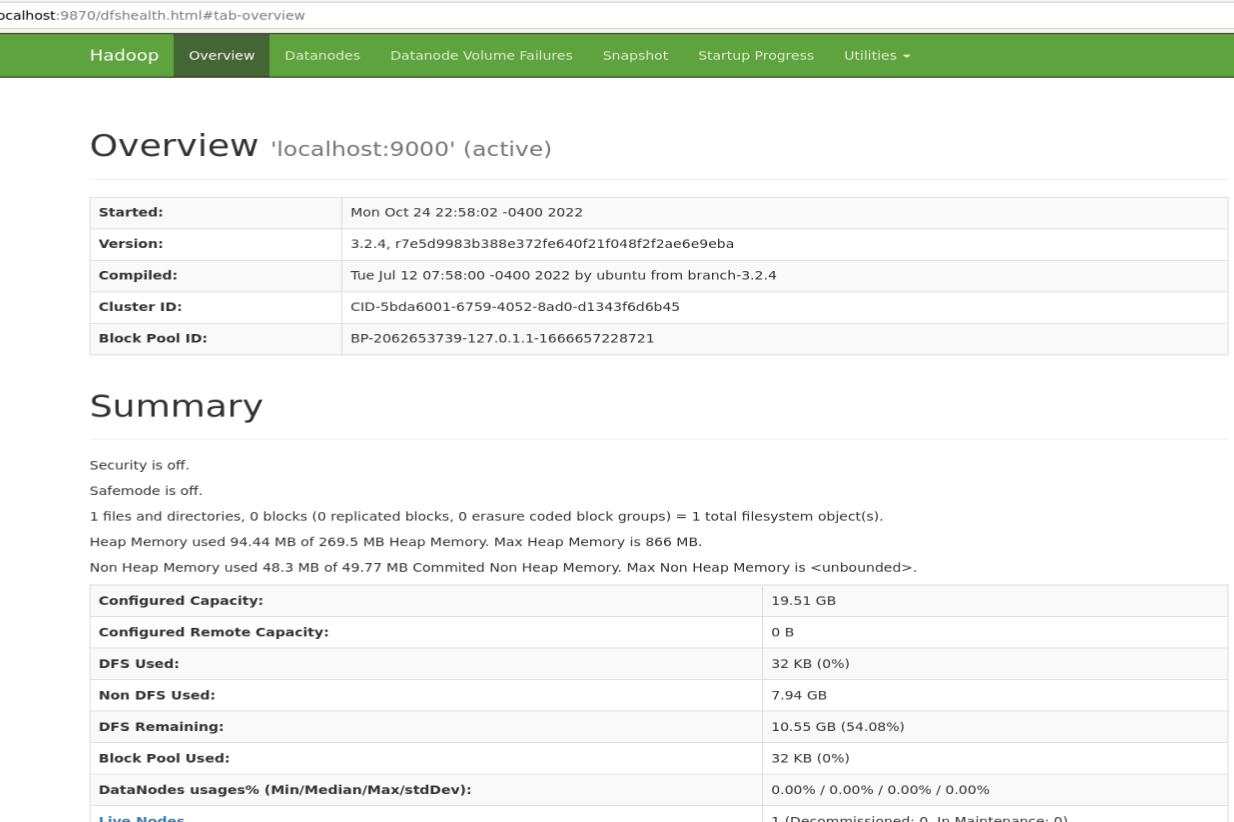
\includegraphics[width=\linewidth]{hadoop_gui2.png}
    \caption{Hadoop Overview GUI - part2}
    \label{fig:hadoopgui2}
\end{figure}

\begin{figure}
    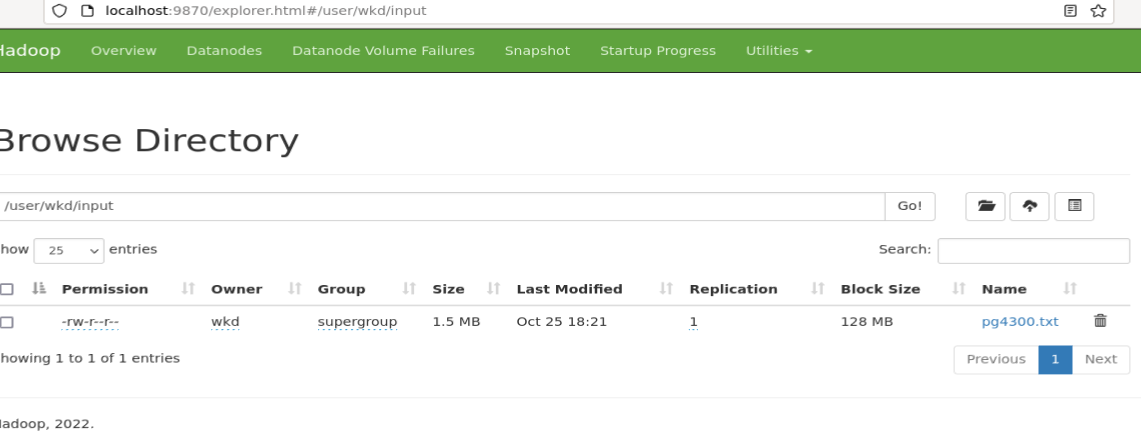
\includegraphics[width=\linewidth]{hadoop_gui3.png}
    \caption{Hadoop directory}
    \label{fig:hadoopgui3}
\end{figure}

\subsection{Performance comparison of Hadoop vs. Linux}
In this part, we compared the word frequency computation capabilities of Hadoop with those of a standard PC running Linux. \newline
First we installed Hadoop and spark binaries.
Then we ran the wordcount program with hadoop on a copy of James Joyce’s Ulysses book page 4300 available at [1]. The wordcount program just counts how many times each word appears in a file. We also di the same on an AWS M4.Large instance using the command cat ./pg4300.txt $\vert $tr ' ' '\textbackslash n' $\vert $sort $\vert $uniq -c. Here are the results:
\begin{table}[h!]
    \caption{Hadoop vs Linux Wordcount}
    \label{tab:table1}
    \begin{tabular}{|l|r|}
        \hline
        \textbf{Hadoop} & \textbf{Linux}\\
        5.961s & 0.170s\\
        \hline
    \end{tabular}
\end{table}

\vspace*{0.5cm}
\noindent
As we can see, Linux completes the task more quickly than Hadoop. This is expected because Hadoop is acceptable or suitable for more sophisticated tasks than the one we used.

\subsection{Performance comparison of Hadoop vs. Spark on AWS}
We first set up our infrastructure as follows in order to compare the performances of Hadoop and Spark on AWS. We generated a M4.large linux Ubuntu instance , and we installed Hadoop 3.3.4 and Spark on it. We confirm the installation of all necessary packages. Then, we timed the WordCount program's execution on both Hadoop and Spark machines three times across the entire dataset. We used 9 text files for this comparison, they can be found in the Datasets folders in Lab2, index shown in Figure~\ref{fig:dataset}.
\begin{figure}
    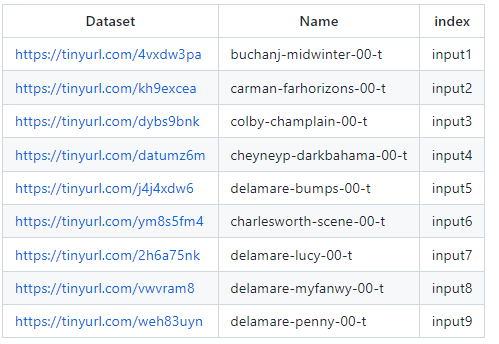
\includegraphics[width=\linewidth]{dataset.png}
    \caption{Dataset index}
    \label{fig:dataset}
\end{figure}

\vspace*{0.5cm}
\noindent
Spark was anticipated to be considerably faster than Hadoop since it makes use of random access memory and this is the case indeed.
The results are shown in the Figure~\ref{fig:plots}.
\begin{figure}
    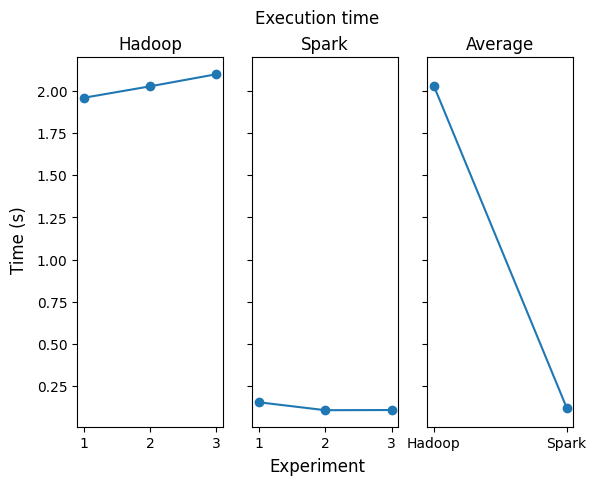
\includegraphics[width=\linewidth]{execution_time.png}
    \caption{Performance comparison of Hadoop and Spark}
    \label{fig:plots}
\end{figure}

\vspace*{0.5cm}
\noindent
This experiment and the last one has been automated through a bash script described in the section~\ref{instructions}.

\section{Instructions to run the code}  \label{instructions}

The entry point of the project is the bash script \textbf{run.sh} located at the root level of Lab2 folder. What this script does is simply to schedule all steps that need to be done in order to have the performance results.
First, it checks whether the necessary credentials (aws\_access\_key\_id, aws\_secret\_access\_key, aws\_session\_token) and the region config are set. The check proceeds this way :
\begin{itemize}
\item Check if the default values have been set by aws cli by means of configure command,
\item If not, check if they are available among the environment variables,
\item If they aren't, get them from user input and export them to make them available for upcoming scripts.
\end{itemize}
Once credentials and minimum config are set, we create and activate a python virtual environment to install dependencies so that user python environment remains unchanged. Then, we deploy and setup infrastructure, it is composed of one M4.Large instance and a security group to allow SSH access. If the setup fails to complete, we teardown already created infrastructure and exit. During the setup we store SSH private key and public IP address for later use.

\vspace*{0.5cm}
\noindent
Infrastructure step completed, we go to the next one which is executing hadoop and spark programs via SSH (using paramiko python library), saving execution time to files (results.txt for hadoop vs linux, hadoop.txt for hadoop performance and spark.txt for spark performance) that are also retrieved by SSH. We save those results in files and plot them. Finally, as soon as we have all we wanted, the infrastructure is destroyed and the virtual environment deactivated.

\begin{justifying}
\section{Social media problem}
\subsection{Input file}
The input file has the following format:\\
userID of a user, followed by a TAB character, followed by the ids of the friends of the user separated by a comma. For example,\\
1\space\space\space2,3\\
3\space\space\space1,2\\
means that user 1 is friends with user 2 and 3, and user 3 is friends with user 2 and 1. Each user and their friends is on a different line (separated by a ENTER character).

\subsection{Map using Hadoop (Java)}
In the map() function, Hadoop automatically splits the input file into lines. The function responsible for this is \\ \verb|MutualFriends.FriendOfFriendsMapper.map(Object key, Text value, Context context)|
\\ This function receives a value containing a string in the format of \verb|userID+TAB+list of friends|\\\verb|separated by a comma|, for example \verb|1TAB2,3,4|, or if the user didn't add anyone, it will look like \verb|1TAB|. The map functions works by 
\begin{enumerate}
    \item Splitting the value by the TAB character, which will result an an array of strings in the format of \verb|[characters before the TAB, characters after the TAB]|. If there are no characters following the TAB, the array will have the format of  \verb|[characters before the TAB]|. For example, if the value is \verb|1TAB2,3,4|, the array will be \verb|["1", "2,3,4"]|; if the value is \verb|1TAB|, the array will be \verb|["1"]|
    \item if the array resulting from splitting by the TAB character have a length of 1, that means the user did not add any friends yet. The key and the sent to the reducer will be
    \begin{enumerate}
        \item key \space\space  = user ID
        \item value             = user ID + TAB + null
    \end{enumerate}
    For example, if the value is "1TAB", the output to the reducer will be
    \begin{enumerate}
        \item key \space\space  = 1
        \item value             = 1TABnull
    \end{enumerate}
    \item if the array resulting from splitting by the TAB character has a length of more than 1, it means the user added at least some friends. The map function will then create a variable  \verb|friendList = user ID + TAB + friends of user ID|. Then, for every user \verb|u| that the user with \verb|user ID| has added (the list can be obtained by splitting the second value of the array by the character ,), the mapper will output to the reducer
    \begin{enumerate}
        \item key \space\space  = u
        \item value             = friendList
    \end{enumerate}
    For example, if the array is ["1", "2,3,4"], the mapper will output
    \begin{enumerate}
        \item key \space\space  = 2
        \item value             = 1TAB2,3,4
        \item key \space\space  = 3
        \item value             = 1TAB2,3,4
        \item key \space\space  = 4
        \item value             = 1TAB2,3,4
    \end{enumerate}
    This ensures that the reducer will have every user along with all their friends of friends, and from which friend they come from. For example, if we have
    \begin{enumerate}
        \item 1 TAB 2,3,4,5
        \item 6 TAB 2,3,4,5,7
    \end{enumerate}
    For the user 2, the reducer will see
    \begin{enumerate}
        \item key = 2; value = 1TAB2,3,4,5
        \item key = 2; value = 6TAB2,3,4,5,7
    \end{enumerate}
    From this, we see that 2 can reach 2,3,4,5 via 1, and 2 can reach 2,3,4,5,7 via 6.
\end{enumerate}
\subsection{Reduce with Hadoop (Java)}
The reducer collects, for each user, all their friends of friends along with from which friend these come from. For example, if 2 can reach 3 via 1 and 4, then 2 and 3 have two mutual friends, namely 1 and 4. The reduce function basically counts how many times a user ID appears in this lists, and returns the ones that appear most often after removing the ones that the user have already added. If the friend list contains null, the reducer outputs an empty list of suggestions. If not, the following steps will be taken: for example, if we have
\begin{itemize}
    \item key \space \space \space = 2
    \item value = 1TAB2,3,4,5
\end{itemize}
Let \verb|alreadyAdded| be a hashset of hashsets of strings that contains all the users that 2 has already added and \verb|mutualFriendsCount| be a HashMap that uses a HashSet of strings as a key and an integer as value. The steps executed by the reducer will be the following (same steps for each value corresponding to 2):
\begin{enumerate}
    \item The string \verb|1TAB2,3,4,5| is splitted by tab to get \verb|["1", "2,3,4,5"]|, and the value \verb|"2,3,4,5"| is splitted by \verb|,| to get the array \verb|potentialFriends = [2, 3, 4, 5]|
    \item The reducer will add \verb|HashSet[(2)]| and \verb|HashSet[(2,1)]| in \verb|alreadyAdded| since 2 cannot add 2 and 2 has already added 1.
    \item  For each user \verb|u| in the list \verb|potentialFriends|, a \verb|HashSet h = HashSet([2,u])| will be created. If h is already in \verb|mutualFriendsCount|, it will be added as a key with a value of 1. If it's already added, we will increase its value by 1.
\end{enumerate}
After all the values associated with 2 have been processed, the keys contained in \verb|alreadyAdded| will be removed from \verb|mutualFriendsCount|. The rest will be stored in an array of \verb|Pair| objects, with a \verb|count| attribute that indicates the number of mutual friends and a \verb|uid| attribute that indicates the user ID. The array is then sorted by \verb|Pair.count| (descending order) then by \verb|Pair.uid| (ascending order). The uid of the 10 first Pair objects (or the whole array, if less than 10 friends of friends) will be returned. Example:
\begin{itemize}
    \item key \space \space \space = 2
    \item value = 1TAB2,3,4,5
    \item value = 6TAB4,3,7,5
    \item value = 8TAB6,3,4,5
\end{itemize}
After processing all the values, \verb|alreadyAdded| will contain
\begin{python}
HashSet([
    HashSet([2]),
    HashSet([2, 1]),
    HashSet([2, 6]),
    HashSet([2, 8])
])
\end{python}
And \verb|mutualFriendsCount| will contain
\begin{python}
HashMap([
    HashSet([2   ]): 1,
    HashSet([2, 1]): 1,
    HashSet([2, 3]): 3,
    HashSet([2, 4]): 2,
    HashSet([2, 5]): 3,
    HashSet([2, 6]): 2,
    HashSet([2, 7]): 1,
    HashSet([2, 8]): 1,
])
\end{python}
After removing the contents of \verb|alreadyAdded| from \verb|mutualFriendsCount|, \verb|mutualFriendsCount| will contain
\begin{python}
HashMap([
    HashSet([2, 3]): 3,
    HashSet([2, 4]): 2,
    HashSet([2, 5]): 3,
    HashSet([2, 7]): 1,
])
\end{python}
And an array containing
\begin{python}
array = [
    Pair{uid="3", count= 3},
    Pair{uid="4", count= 2},
    Pair{uid="5", count= 3},
    Pair{uid="7", count= 1},
]
\end{python}
will be produced, then sorted first according to count, then according to uid (ex. "3" comes before "5" because 3 < 5, even though they both have three mutual friends with 2):
\begin{python}
array = [
    Pair{uid="3", count= 3},
    Pair{uid="5", count= 3},
    Pair{uid="4", count= 2},
    Pair{uid="7", count= 1},
]
\end{python}
The output will be
\begin{itemize}
    \item key = 2
    \item value = 3,5,4,7
\end{itemize}

\subsection{Result}
For the following users, we have:\\
924 \space \space \space \space439,2409,6995,11860,15416,43748,45881\\
8941\space \space \space \space8943,8944,8940\\
8942\space \space \space \space8939,8940,8943,8944\\
9019\space \space \space \space9022,317,9023\\
9020\space \space \space \space9021,9016,9017,9022,317,9023\\
9021\space \space \space \space9020,9016,9017,9022,317,9023\\
9022\space \space \space \space9019,9020,9021,317,9016,9017,9023\\
9990\space \space \space \space13134,13478,13877,34299,34485,34642,37941\\
9992\space \space \space \space9987,9989,35667,9991\\
9993\space \space \space \space9991,13134,13478,13877,34299,34485,34642,37941\\
All the users have received either 10 recommendations or as many as possible. For example, one of the result is\\
0\space \space \space \space38737,18591,27383,34211,337,352,1532,12143,12561,17880\\
we can verify manually that 0 and 38737 have 5 friends in common, and 0 and 18591 have
4 mutual friends in common, and so on.

\subsection{How to run the program}
All the code for running the program is in compile.sh. The only parts that need to be changed
manually is the input and the output directory, along with the hadoop path (if necessary). To
run compile.sh, just type ./compile.sh in its directory.\\
However, if it does not work, it can be ran this way (code based on Apache Hadoop word count tutorial, 2022):

\begin{python}
rm -r path/to/output
export JAVA_HOME="/path/to/java/"
export PATH=${JAVA_HOME}/bin:\${PATH}
export HADOOP_CLASSPATH=\${JAVA_HOME}/lib/tools.jar
/path/to/hadoop/bin/hadoop com.sun.tools.javac.Main MutualFriends.java Pair.java
jar cf tp2.jar *.class
/path/to/hadoop/bin/hadoop jar tp2.jar MutualFriends /path/input /path/output
\end{python}

\subsection{Results on Azure}
We also run this program on Azure (this is a screenshot of the content of the output file):
\begin{enumerate}
    \item Create a Linux virtual machine with the following setup in the "basic" section (the rest can be left to default settings): 
    \begin{python}
    name of the virtual machine: mapreduce
    availability region: (Canada) Canada central
    Select inbound ports: HTTP, SSH, HTTPS
    Username: can be anything
    key pair name: can be anything    
    \end{python}
    
\begin{figure}[H]
    \centering
    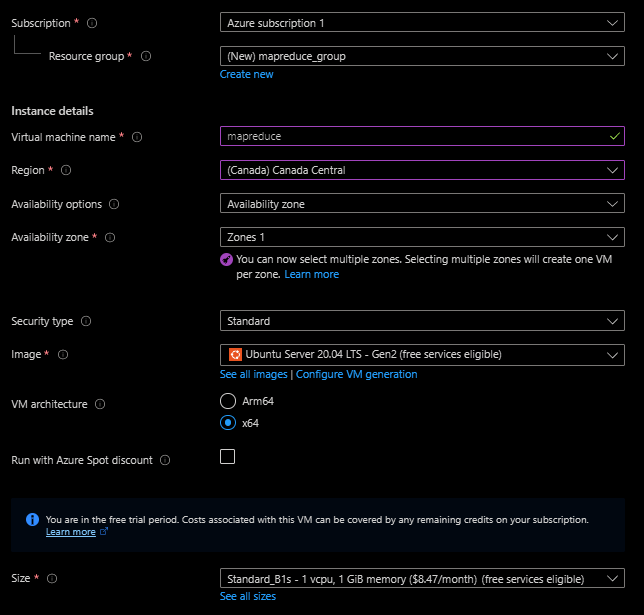
\includegraphics[width=\linewidth]{azure-setup1.PNG}
    \caption{Basic configuration}
    \label{fig:mrazure}
\end{figure}

\begin{figure}[H]
    \centering
    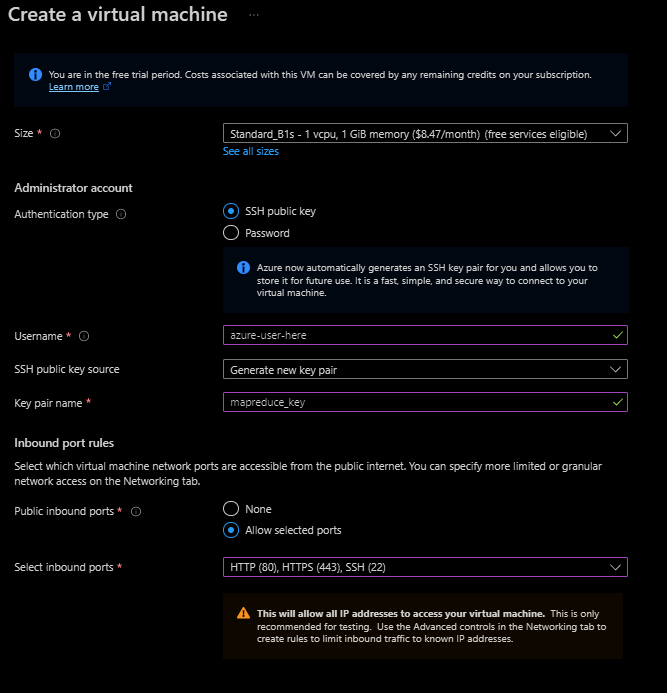
\includegraphics[width=\linewidth]{azure-setup2.PNG}
    \caption{Basic configuration (next section)}
    \label{fig:mrazure}
\end{figure}

    \item For disks, select "Standard HDD" for better cost. The rest of the options can be left as default (Networking,Management, Monitoring, Advanced, Tags).

\begin{figure}[H]
    \centering
    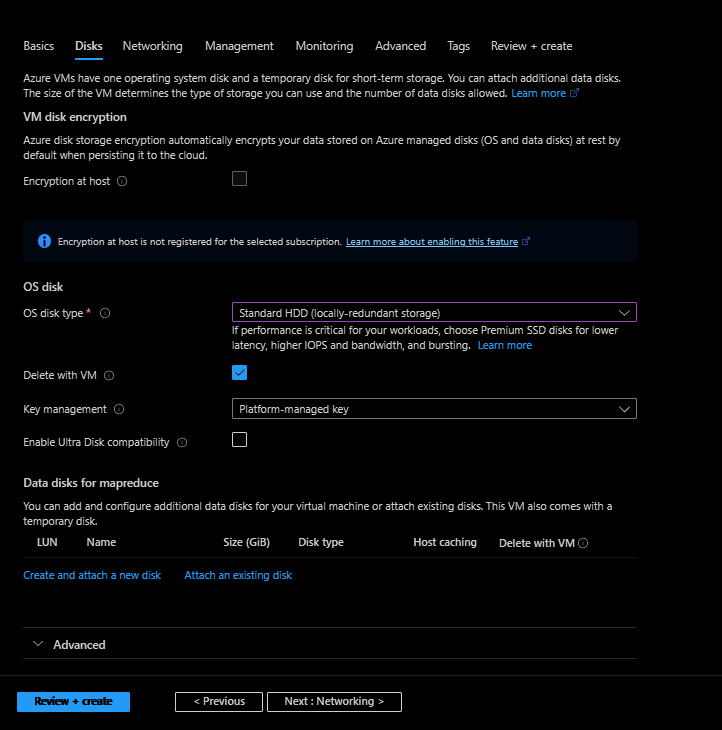
\includegraphics[width=\linewidth]{azure-disk.PNG}
    \caption{Disk configuration}
    \label{fig:mrazure}
\end{figure}

    \item After the machine is up and running, an SSH key pair is generated on a local linux machine, and the public key of the virtual machine (on Azure) is updated using the "reset password" functionality
\begin{figure}[H]
    \centering
    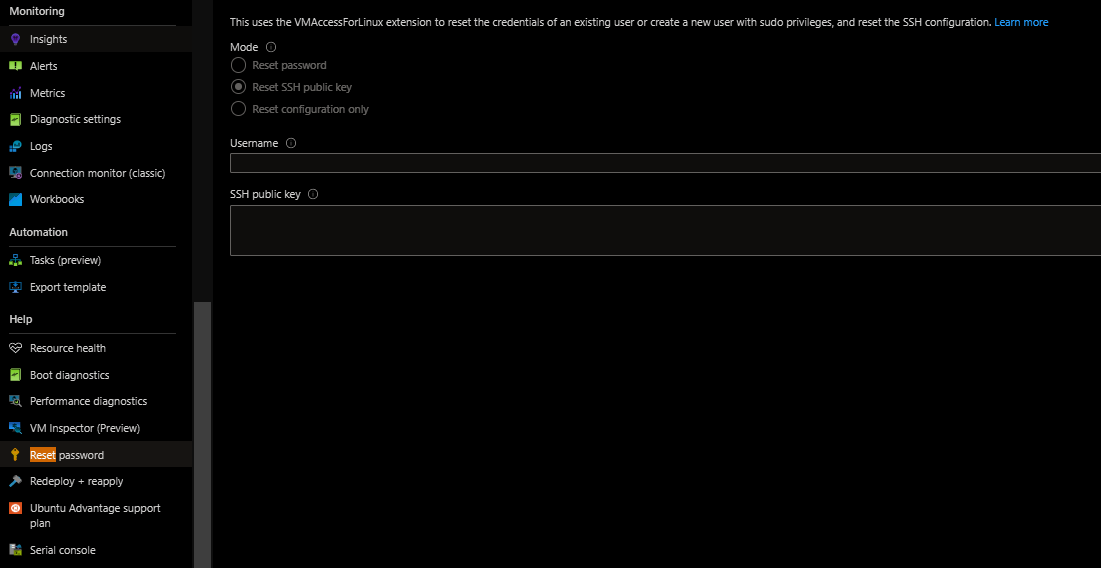
\includegraphics[width=\linewidth]{Azure-reset-ssh.PNG}
    \caption{Changing public key (public key not shown for security reasons)}
    \label{fig:mrazure}
\end{figure}
    \item the following commands are used to connect to the VM:
    \begin{lstlisting}[language=Bash]
# on a local machine (step 3)
chmod 400 path/to/private_key.pem
ssh -i path/to/private_key.pem <azure user name>@<public IP of VM>

# on the Azure Virtual machine
sudo apt-get update
sudo apt-get install openjdk-17-jre-headless
export JAVA_HOME="/path/to/java"
sudo wget <link to hadoop version>
sudo tar -xvzf path/to/hadoop.tar.gz

# on the local machine
sudo scp -i path/to/private/key tp2.jar \
    <azure user name>@<public IP of VM>:/home/azureuser
sudo scp -i path/to/compile.sh \
    <azure user name>@<public IP of VM>:/home/azureuser
./compile.sh
\end{lstlisting}
\end{enumerate}

\begin{figure}[H]
    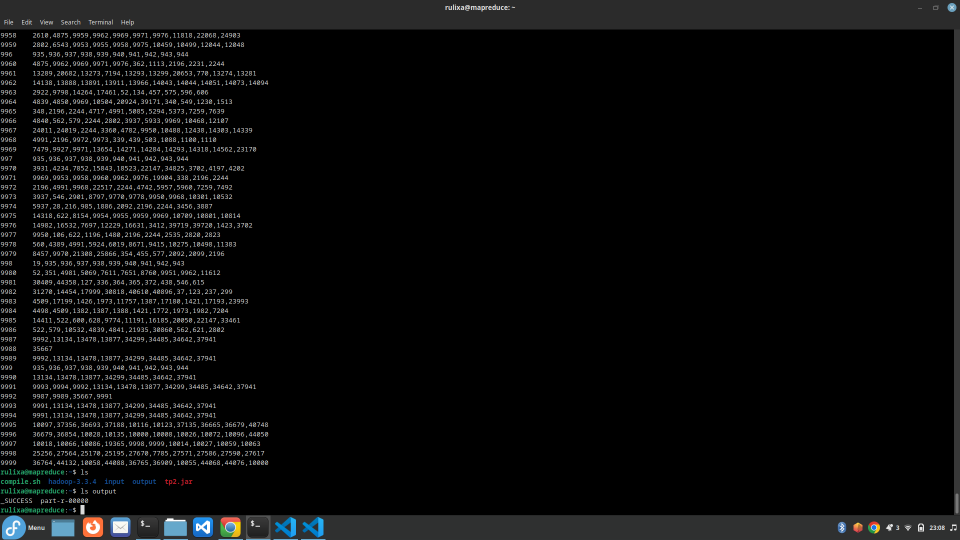
\includegraphics[width=\linewidth]{azure.png}
    \caption{Output of MapReduce from Microsoft Azure}
    \label{fig:mrazure}
\end{figure}

\end{justifying}

\section{References}
[1] Gutenberg textual data. http://www.gutenberg.org/cache/epub/4300/pg4300.txt.\newline
[2] Github repo. https://github.com/MichelleSS1/Lab8415\newline
[3] Apache Software Foundation. (2022, July 29). {\it{Mapreduce tutorial}}. Apache Hadoop. Retrieved November 4, 2022, from https://hadoop.apache.org/docs/stable/hadoop-mapreduce-client/hadoop-mapreduce-client-core/MapReduceTutorial.html 

\end{document}
